% \clearpage
\section{Experiments}

% In this section, we evaluate the proposed ASVD method.
% We use one Nvidia RTX A6000 to execute our experiments.
% We use the code and model downloaded from huggingface-hub.
In this section, we assess the effectiveness of \asvd~by conducting experiments on LLaMA~\citep{touvron2023llama1} and LLaMA-2~\citep{touvron2023llama2}, and presenting results on various tasks, such as Perplexity in WIKI~\citep{merity2016pointer} and MMLU~\citep{hendrycks2020measuring}. 

% \subsection{Hyper-parameters Exploration}

% In our study, we initiate an exploration of hyper-parameters in \asvd, focusing on the activation channel significance metric and the control factor $\alpha$. This exploration is conducted on OPT-125m, a relatively small network that facilitates rapid evaluation.
% We rigorously explored the control factor $\alpha$, and two methods for quantifying activation significance: Absolute Mean Value of Input Activation and Absolute Maximum Value of Input Activation. 
% \underline{More details can be found in the Appendix.} 
% In summary, based on our explorations, we chose $\alpha=0.5$ and the Absolute Mean Value method for setting the scaling matrix $S$ in the \asvd~process in the following experiments.




% Next, we evaluate the ASVD on LLaMA-7b and LLaMA-2-7b, which contains 7 billion of parameters.
% For each model, we also sample 16 calibration data with 2048 tokens from the wikitext dataset.
% Then we evaluate the sensitivity of each layer.
% To overview how the compression impact on model performance, we set different threshold for truncation rank searching to compress the network.
% The compressed networks takes different compression ratios. And we evaluate them to get the perplexity of wikitext2 and ptb.
% Then we plot the parameter ratio-perplexity line of these compressed networks.
% The results are demonstrated in Figure~\ref{im_ppl}.
% We can observe from the plot that 1. the perplexity increase as the parameter ratio increase because xxx. 2. there are a plain area above 0.9 parameter ratio, in these area ASVD decompose the less sensitive layers, their decomposition don't affect the prediction accuracy. 3. when the parameter ratio < 0.85, the perplexity increase quickly, that means sensitive layers are decomposed to a lower truncation rank.

\subsection{Settings}
We conducted a comprehensive evaluation of Activation-aware Singular Value Decomposition (\asvd) on two series of Large Language Models (LLMs): LLaMA and LLaMA-2 \citep{touvron2023llama1,touvron2023llama2}. Our experiments encompassed models ranging from 7 billion to 13 billion parameters. For each model, we selected a calibration set with 32 samples, and each sample contains 2048 tokens, from the Wikitext dataset to assess the layer-wise sensitivity. We explore two methods to set transform matrix $\mathbf{S}$. The first is the magnitude-based method (Eq.\ref{eq:set_matrix_magnitude}), which is indicated by \asvd. We set $\alpha$ to 0.5 in our experiments~\footnote{The exploration of hyper-parameter $\alpha$ can be found in the Appendix.}. We also experimented with the Cholesky decomposition method (Eq.\ref{eq:set_matrix_cholosky}) to set the transform matrix, denoted \asvd+ in our experiments.

\subsection{Parameters Compression}

% \begin{table}[t]
% \centering
% \caption{Perplexity on Wikitext2 for exploring hyper-parameters on OPT-125m.}
% \label{tab_explore_param}
% \resizebox{0.5\linewidth}{!}{
% \begin{tabular}{@{}cccccc@{}}
% \toprule
% $\alpha$         & 0.1     & 0.25    & 0.5     & 1       & 2       \\ \midrule
% SVD+STRS      & \multicolumn{5}{c}{103.39}                      \\
% ASVD abs mean & 47.54 & 37.12 & \textbf{36.89} & 41.53 & 43.81 \\
% ASVD abs max  & 52.63 & 47.17 & 40.14 & 41.94 & 52.55 \\ \bottomrule
% \end{tabular}
% }
% % \vspace{-0.15in}
% \end{table}

\begin{figure}[tb]
    \centering
    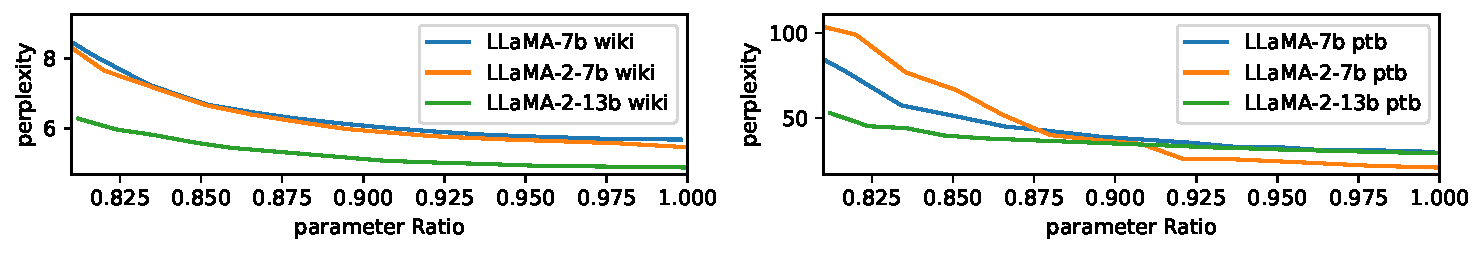
\includegraphics[width=0.95\textwidth]{ims/ppl_plot.pdf}
    \vspace{-0.05in}
    \caption{Perplexity trends of \asvd~compression on LLaMA-2-13b, LLaMA-2-7b and LLaMA-7b.}
    \vspace{-0.1in}
    \label{im_ppl}
\end{figure}

\begin{table}[tb]
\centering
\caption{Performance under various compression scenarios. Param ratio indicates the proportion of parameters remaining after decomposition. MMLU results are 0-shot. SVD* means SVD using Sensitivity-based Truncation Rank Searching.}
\label{tab_llama_eval}
\resizebox{1\linewidth}{!}{
\begin{tabular}{@{}cc|ccc|ccc|ccc@{}}
\toprule
         &             & \multicolumn{3}{c|}{LLaMA-7b} & \multicolumn{3}{c|}{LLaMA-2-7b} & \multicolumn{3}{c}{LLaMA-2-13b} \\ \midrule
method   & param ratio & MMLU     & wiki     & ptb     & MMLU      & wiki    & ptb       & MMLU      & wiki     & ptb      \\ \midrule
original & 1           & 30.76\%  & 5.68     & 29.63   & 34.86\%   & 5.47    & 20.82     & 40.16\%   & 4.88     & 29.21    \\
SVD      & 0.95        & 22.98\%  & 2800  & 5458 & -         & nan     & nan       & -         & nan      & nan      \\
SVD* & 0.95        & 23.92\%  & 136.05   & 183.92  & 24.78\%   & 46.79   & 363.37    & 24.86\%   & 167.63   & 567.02   \\
SVD* & 0.9         & 23.54\%  & 698.66   & 262.03  & 24.31\%   & 114.45  & 27660  & -         & nan      & nan      \\ \midrule
\asvd~    & 0.95        & 30.26\%  & 5.78     & 32.64   & 33.24\%   & 5.64    & 23.98     & 39.52\%   & 4.94     & 31.93    \\
\asvd~    & 0.9         & 29.67\%  & 6.09     & 37.80   & 32.58\%   & 5.93    & 32.63     & 40.04\%   & 5.12     & 34.03    \\
\asvd~    & 0.85        & 29.70\%  & 6.80     & 52.11   & 31.57\%   & 6.74    & 59.84     & 37.95\%   & 5.54     & 39.32    \\
\asvd~    & 0.8         & 27.85\%  & 8.89     & 88.09   & 28.15\%   & 8.91    & 114.70    & 34.63\%   & 6.53     & 59.68    \\
\asvd~    & 0.75        & 24.94\%  & 14.51    & 212.80  & 25.97\%   & 18.97   & 432.57    & 28.59\%   & 8.71     & 110.10   \\ \bottomrule
\end{tabular}
}
\vspace{-0.1in}
\end{table}

Sensitivity-based Truncation Rank Searching (STRS in Sec.\ref{sec:method-sensitivity}) involves setting varying thresholds binary searching process, enabling us to observe the impact of different compression levels on model performance. This approach resulted in a range of compressed networks, each characterized by a unique compression ratio. 
We evaluated the performance of these compressed networks using perplexity as the primary metric, focusing on two datasets: Wikitext-2 (wiki) and the Penn Treebank (ptb). 
% The objective was to understand the relationship between compression ratio and model performance.
The results, illustrated in Fig.\ref{im_ppl}, reveal several key insights:
(1) As the parameter ratio decreases, there is a corresponding increase in perplexity. 
% As more parameters are compressed, the more error is introduced by SVD. This reduces representational capacity of the network, thereby resulting in higher perplexity scores. 
(2) A plateau region is observed when the parameter ratio exceeds 0.9. In this range, \asvd~predominantly decompresses the less sensitive layers, resulting in minimal impact on prediction accuracy.
(3) Below a parameter ratio~\footnote{parameter ratio 0.85 means compress the model size by 15\%.} of 0.85, there is a rapid increase in perplexity, indicating that the more sensitive layers are being decompressed to a lower truncation rank, adversely affecting the model's performance.

We also present a detailed analysis of the performance of compressed networks at various parameter ratios. 
% This analysis aims to elucidate the impact of different compression techniques on network efficiency and accuracy.
Table~\ref{tab_llama_eval} displays the performance metrics for two LLaMA models, LLaMA-7b and LLaMA-2-7b, under several compression scenarios. These metrics include MMLU zero-shot evaluation, perplexity on the Wikitext dataset (wiki), and perplexity on the Penn Treebank dataset (ptb).
Our observations reveal significant performance variations based on the parameter ratio and the compression method used. Specifically, the table highlights the performance of each model when using standard SVD, SVD with binary search for truncation ranks (SVD*), and \asvd~at different parameter ratios ranging from 0.75 to 0.95.

We compare \asvd~ and \asvd+\footnote{\asvd+ refer to \asvd~with whitening method for obtaining the transformation matrix in Eq.\ref{eq:set_matrix_cholosky}} with SVD-LLM~\citep{wang2024svdllm}. 
% The results are shown in Table~\ref{table:asvd_plus}. From this table, we observe that \asvd+ can improve the performance of \asvd, especially when the compression ratio is high.
The results in Table~\ref{table:asvd_plus} show that \asvd+ can improve the performance of \asvd, especially when the compression ratio is high.
\asvd+ also outperforms the SVD-LLM method, particularly when the compression ratio is less than 30\%. 
% This is because SVD-LLM does not consider the layer-wise differences. While our method uses Sensitivity-based Truncation Rank Searching to set each layer with different compression ratio. 
This is because SVD-LLM does not consider the layer-wise differences. In contrast, our method uses Sensitivity-based Truncation Rank Searching to set each layer with a different compression ratio. 
However, when the compression ratio is larger than 30\%, all of these methods can significantly improve the perplexity of the LLMs.

\begin{table}[tb]
\centering
\caption{The perplexity on wikitext2 of SVD-LLM, \asvd~ and \asvd+. In this table, we take the setting of SVD-LLM that the lm head is not taken into consideration to compute the param ratio.}
\label{table:asvd_plus}
\resizebox{0.8\linewidth}{!}{
\begin{tabular}{@{}cccc|cccc@{}}
\toprule
\multicolumn{4}{c|}{LLama-2-7b}                                      & \multicolumn{4}{c}{LLama-2-13b}                                      \\ \midrule
Param ratio & SVD-LLM & \asvd & \asvd+ & Param ratio & SVD-LLM & \asvd & \asvd+ \\ \midrule
0.95        & 6.93    & 5.64                 & 5.56                  & 0.95        & 5.70    & 4.94                 & 4.93                  \\
0.9         & 7.27    & 5.93                 & 5.74                  & 0.9         & 5.94    & 5.12                 & 5.03                  \\
0.85        & 7.76    & 6.74                 & 6.10                  & 0.85        & 6.24    & 5.54                 & 5.26                  \\
0.8         & 8.38    & 8.91                 & 6.86                  & 0.8         & 6.66    & 6.53                 & 5.77                  \\
0.75        & 9.30    & 18.97                & 8.38                  & 0.75        & 7.22    & 8.71                 & 6.54                  \\
0.7         & 10.67   & 159.21               & 10.62                 & 0.7         & 8.00    & 20.82                & 7.82                  \\
0.65        & 12.82   & 1034.59              & 13.87                 & 0.65        & 9.10    & 53.30                & 9.84                  \\
0.6         & 16.14   & 730.60               & 19.12                 & 0.6         & 10.78   & 133.88               & 13.18                 \\ \bottomrule
\end{tabular}
}
\end{table}

\subsection{KV Cache Compression}

\begin{table}[tb]
\centering
\caption{Performance under different KV cache compression ratio.}
\label{table:kv_cache_compression}
\resizebox{0.9\linewidth}{!}{
\begin{tabular}{@{}ccccccccccc@{}}
\toprule
                             &         & \multicolumn{9}{c}{KV cache ratio}                                          \\ \midrule
model                        & dataset & 1(original) & 0.9   & 0.8   & 0.7   & 0.6   & 0.5   & 0.4   & 0.3   & 0.2   \\ \midrule
\multirow{2}{*}{LLaMA-2-7b}  & wiki    & 5.47        & 5.46  & 5.48  & 5.50  & 5.55  & 5.67  & 5.94  & 6.55  & 8.71  \\
                             & ptb     & 20.82       & 21.04 & 21.52 & 21.66 & 21.91 & 22.16 & 24.33 & 26.89 & 38.72 \\ \midrule
\multirow{2}{*}{LLaMA-2-13b} & wiki    & 4.88        & 4.89  & 4.90  & 4.91  & 4.92  & 4.96  & 5.08  & 5.33  & 6.06  \\
                             & ptb     & 29.21       & 29.64 & 29.95 & 30.21 & 30.99 & 31.69 & 34.03 & 36.61 & 47.24 \\ \bottomrule
\end{tabular}
}
\vspace{-0.1in}
\end{table}

We evaluate the KV Cache compression by using \asvd~to decompose k projection and v projection in transformer~\citep{vaswani2017attention}.
Table~\ref{table:kv_cache_compression} summarizes the results, showing the perplexities on the wikitext2 and Penn Treebank datasets for different KV cache compression ratios. It is evident that the perplexity values remain stable when the KV cache ratio is above 40\%. 
When the ratio is lower than 40\%, the performance of the network is decreased.
These observations suggest that \asvd~is effective to compress the KV cache without negatively impacting the model. 

\subsection{Integrating \asvd~with Quantization}
\label{sec:quantization}

\begin{table}[tb]
\centering
\caption{Combining weight quantization with \asvd. Param ratio indicates the proportion of parameters remaining after \asvd, with 1 implying no decomposition.}
\label{tab_asvd_quant}
\resizebox{0.9\linewidth}{!}{
\begin{tabular}{@{}ccccccccccc@{}}
\toprule
\multicolumn{1}{c|}{}            & \multicolumn{5}{c|}{LLaMA-2-7b}                                                                                                                                                                          & \multicolumn{5}{c}{LLaMA-2-13b}                                                                                                                                                    \\ \midrule
\multicolumn{1}{c|}{param ratio} & FP16  & \begin{tabular}[c]{@{}c@{}}INT8\\ (RTN)\end{tabular} & \begin{tabular}[c]{@{}c@{}}INT8\\ (AWQ)\end{tabular} & NF4    & \multicolumn{1}{c|}{\begin{tabular}[c]{@{}c@{}}INT4\\ (AWQ)\end{tabular}} & FP16  & \begin{tabular}[c]{@{}c@{}}INT8\\ (RTN)\end{tabular} & \begin{tabular}[c]{@{}c@{}}INT8\\ (AWQ)\end{tabular} & NF4   & \begin{tabular}[c]{@{}c@{}}INT4\\ (AWQ)\end{tabular} \\ \midrule
\multicolumn{11}{c}{wiki}                                                                                                                                                                                                                                                                                                                                                                                                        \\ \midrule
\multicolumn{1}{c|}{1}           & 5.47  & 5.48                                                 & 5.45                                                 & 5.65   & \multicolumn{1}{c|}{5.59}                                                 & 4.88  & 4.88                                                 & 4.88                                                 & 4.98  & 4.97                                                 \\
\multicolumn{1}{c|}{0.95}        & 5.64  & 5.64                                                 & 5.56                                                 & 5.83   & \multicolumn{1}{c|}{5.82}                                                 & 4.94  & 4.95                                                 & 4.97                                                 & 5.08  & 5.18                                                 \\
\multicolumn{1}{c|}{0.9}         & 5.93  & 5.94                                                 & 5.82                                                 & 6.2    & \multicolumn{1}{c|}{6.21}                                                 & 5.12  & 5.11                                                 & 5.15                                                 & 5.31  & 5.43                                                 \\
\multicolumn{1}{c|}{0.85}        & 6.74  & 6.73                                                 & 6.51                                                 & 7.43   & \multicolumn{1}{c|}{7.18}                                                 & 5.54  & 5.56                                                 & 5.59                                                 & 5.9   & 5.96                                                 \\ \midrule
\multicolumn{11}{c}{ptb}                                                                                                                                                                                                                                                                                                                                                                                                         \\ \midrule
\multicolumn{1}{c|}{1}           & 20.82 & 20.82                                                & 20.93                                                & 22.7   & \multicolumn{1}{c|}{21.50}                                                & 29.15 & 29.12                                                & 29.29                                                & 30.31 & 30.47                                                \\
\multicolumn{1}{c|}{0.95}        & 23.98 & 23.95                                                & 25.47                                                & 35.91  & \multicolumn{1}{c|}{27.79}                                                & 31.93 & 31.67                                                & 30.19                                                & 33.89 & 31.21                                                \\
\multicolumn{1}{c|}{0.9}         & 32.63 & 32.19                                                & 37.11                                                & 40.82  & \multicolumn{1}{c|}{39.31}                                                & 34.03 & 33.64                                                & 35.47                                                & 34.93 & 38.95                                                \\
\multicolumn{1}{c|}{0.85}        & 59.84 & 63.76                                                & 84.52                                                & 427.59 & \multicolumn{1}{c|}{95.85}                                                & 39.32 & 40.02                                                & 43.01                                                & 44.49 & 50.56                                                \\ \bottomrule
\end{tabular}
}
% \vspace{-0.4in}
\end{table}

This section investigates the compatibility of \asvd~with quantization techniques for compressing LLMs. We explore the integration of \asvd~with different quantization methods. 
Simple quantization methods include Round-To-Nearest (RTN) and 4-bit NormalFloat (NF4) \citep{dettmers2023qlora}. The advanced LLM quantization method is Activation-aware Weight Quantization (AWQ) \citep{lin2023awq}. 
Note that our study focuses on establishing the orthogonal property of ASVD to these basic quantization methods. Future work could extend this investigation to more advanced quantization techniques and other LLM compression approaches.
Our experimental framework involves two stages. Firstly, we apply \asvd~to decompose the network. Subsequently, we quantize the decomposed weights. 
% We employ per-channel asymmetric quantization, targeting two quantization levels: 8-bit and 6-bit. We employ NF4 for quantizing to 4-bit. 
% The impact of these quantization levels on network performance is then assessed.

Table~\ref{tab_asvd_quant} summarizes the results of our experiments on LLaMA-2-7b, LLaMA-2-13b models~\citep{touvron2023llama2}. The following observations were made: \textbf{8-bit Weight Quantization:} The results indicate that 8-bit quantization has a negligible impact on model performance, both for the original and the ASVD-compressed networks. 
% \textbf{6-bit Quantization:} A slight degradation in prediction accuracy is observed with 6-bit quantization. This effect is more pronounced in networks with higher compression (lower parameter ratios), suggesting a compounded impact of compression and lower bit quantization.
\textbf{4-bit weight Quantization:} Upon quantizing the network into NF4 and INT4(AWQ), a further deterioration in prediction accuracy is observed. When param ratio is greater than 0.9, the performance decline attributed to quantization is approximately consistent with that of the non-decomposed network. 
We observe that the performance degradation of LLaMA-2-13b is less than that of LLaMA-2-7b, indicating that the larger model is more robust to compression.
% For instance, in the case of LLaMA-2-7b without decomposition, the NF4 quantization results in a wiki PPL decrease of 0.18 compared to FP16. Similarly, at a param ratio of 0.95, the NF4 quantization yields a PPL decrease of 0.19 compared to FP16.
In summary, the findings suggest that \asvd~is compatible with weight quantization techniques.
% like RTN. This compatibility is particularly noticeable with 8-bit quantization, where performance is largely preserved. 
% The slight degradation with 6-bit quantization warrants further investigation, especially in the context of more advanced quantization methods.


% \subsection{Quantization and ASVD}

% Quantization is another method to compression large language models.
% In this section, we will evaluate how ASVD can be work together with quantization.
% Because in this paper is not focus on quantization, we only use the simplest quantization method, RTN.
% In the future work, we can explore combine ASVD with more sophisticated methods such as GPTQ or RPTQ.
% For the experiments, we first decompose the network using ASVD.
% Then we quantize the decomposed weights using per-channel round-to-nearest quantization into 8bit or 6bit and then evaluate the results.
% As shown in Table~\ref{tab_asvd_quant}, xxx.
% The 8bit quantization almost not affect the result on both original network and ASVD compressed networks.
% For 6bit quantization there is some prediction accuracy degradation.  
% xxxx (other observations and analyze)
% In conclusion, ASVD can work together with quantization well.



% \subsection{Inference Speed Evaluation}

% As Section~\ref{sec_efficeint_inference} indicated, ASVD can not only reduce the weights storage and weight transferring in LLMs, but also reduce the computation required by LLMs.
% In this section, we will evaluate the inference good by using decomposed network.
% We evaluate the inference speed using , We test on Intel(R) Xeon(R) Gold 6226R CPU @ 2.90GHz (we use num threads=32).

\subsection{Decomposed Network Analysis}


\begin{figure}[tb]
\centering
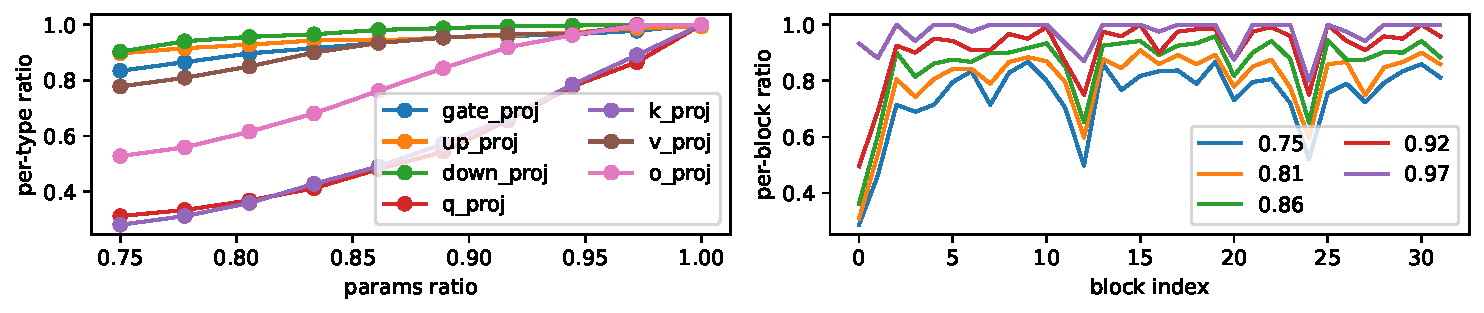
\includegraphics[width=0.95\textwidth]{ims/analysis_meta-llama_Llama-2-7b-hf.pdf}
\vspace{-0.15in}
\caption{Per-type parameters ratio and per-block parameters ratio on LLaMA-2-7b after \asvd~compression.}
\vspace{-0.2in}
\label{im_analysis}
\end{figure}

We conduct a detailed analysis of the decomposed network. Figure~\ref{im_analysis} presents the per-type parameters ratio and per-block parameters ratio.
Observing the plot, we note that parameters in the MLP components (gate projection, up projection, and down projection) exhibit minimal compression. In MHA, the V projection layer experiences relatively small compression, whereas q projection and k projection can be significantly compressed, indicating redundancy in these components.
Turning our attention to the per-block compression ratio, we find that the first layer can undergo substantial compression. In contrast, the compression ratios for the other layers, except for two middle layers, show similar compression rates.

% \subsection{Efficiency Improvement Analysis}
% \label{sec_inference_cost}
% Regarding the computational aspect, let's consider the input matrix $\mathbf{X} \in \mathbb{R}^{n \times t}$ and the weight matrix $\mathbf{W} \in \mathbb{R}^{m \times n}$. In the original linear layer, the matrix multiplication is represented as $\mathbf{Y} = \mathbf{W}\mathbf{X}$. The number of Multiply-Accumulate (MAC) operations, denoted as $C$, in the original linear layer can be computed as: $C = tmn$.
% After the \asvd~decomposition, the matrix multiplication transforms into $\mathbf{Y} = \mathbf{A}_k \mathbf{B}_k$. To analyze the computational efficiency, we calculate the MAC operations, denoted as $C_k$, for this decomposed form. The computation for $C_k$ is given by:
% $C_k = tkm+tkn$

This computation ratio can be expressed as the ratio of $C_k$ to $C$, which is equivalent to the parameter ratio:
\begin{equation}
    \frac{C_k}{C} = \frac{km + kn}{nm}
\end{equation}
Remarkably, this computation ratio mirrors the weight number compression ratio, highlighting the efficient use of computational resources achieved through \asvd. 
In summary, \asvd~can not only reduce the weight storage and weight transferring overheads in LLM deployment but also reduce the computation required by LLM inference. 